\documentclass[a4paper]{article}
\usepackage{cmap}
\usepackage{mathtext}
\usepackage{amssymb}
\usepackage{amsmath}
\usepackage{wrapfig}
\usepackage[russian]{babel}
\usepackage{indentfirst}
\usepackage[pdftex]{graphicx}
\usepackage{multirow}
\usepackage{mathrsfs}
\usepackage{biblatex}
\usepackage{siunitx}
\usepackage[left=2cm,right=2cm,top=2cm,bottom=2cm]{geometry}
\usepackage{fancyhdr}
\bibliography{bib}
\pagestyle{fancy}
\newcommand{\const}{\mathrm{const}}
\newcommand{\rref}[1]{(\ref{#1})}
\newcommand{\isotope}[2]{$ ^{#2}\mathrm{#1} $}
\newenvironment{comment}{}{}
\newcommand{\picref}[1]{рис. \ref{#1}}
\newcommand{\mbf}{\mathbf}
\newcommand{\gmm}{$\gamma $}
\newcommand{\btt}{$\beta $}
\newcommand{\dlt}{$\delta $}
\newcommand{\Equip}[3]{
	
	\item{\bf #1:} $\Delta = \pm #2\; #3$}
\newcommand{\equip}[1]{
	
	\item{\bf #1}}
\newcommand{\labname}{Исследование энергетического спектра \btt-частиц и определение их максимальной энергии при помощи	магнитного спектрометра} 	% название пиши здесь
\newcommand{\labnum}{5.4.2}		% номер вводи здесь
\renewcommand{\epsilon}{\varepsilon}
\renewcommand{\phi}{\varphi}
\newcommand{\angstrom}{\text{\AA}}
\fancyfoot{}
\fancyhead[RE, RO]{\thepage}
\fancyhead[LE, LO]{Лабораторная работа \labnum \space \labname}
\title{Лабораторная работа \labnum \space \labname}
\author{Иван Сладков}
\begin{document}
	\maketitle
	\thispagestyle{empty}
	\section{Аннотация}
	В данной работе проводится исследование энергетического	спектра \btt-частиц при распаде ядер \isotope{Cs}{137} и определяется их максимальная энергия. Калибровка спектрометра осуществляется по энергии электронов внутренней конверсии \isotope{Cs}{137}.
	
	\section{Теоретические сведения}
	
	\begin{wrapfigure}{}{0.49\textwidth}
		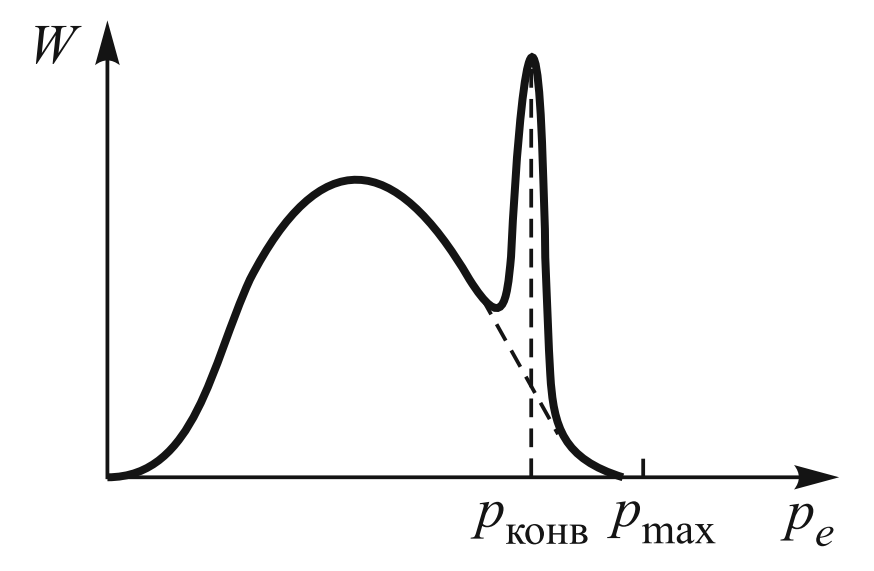
\includegraphics[width=1.0\linewidth]{Screenshot_1}
		\caption{Форма спектра \btt-частиц при разрешённых переходах}
		\label{fig:screenshot1}
	\end{wrapfigure}
	
	Бета-распадом называется самопроизвольное превращение ядер,	при котором их массовое число нс изменяется, а заряд увеличивается или уменьшается на единицу.В данной работе мы будем иметь дело с электронным \btt-распадом:
	\begin{equation*}
		^A_Z X \leftarrow ^A_{Z+1} X+e^-+\widetilde{\nu},
	\end{equation*}
	при котором кроме электрона испускается антинейтрино. 
	
	Выясним вид энергетического спектра \btt-частиц.
	Во-первых, учтём ЗСЭ:
	\begin{equation}\label{eq:ЗСЭ}
		E_e - E - c k = 0,
	\end{equation}
	где $ c k $ -- энергия нейтрино, $ E_e $ -- максимальная энергия электрона, $ E $ -- кинетическая энергия электрона, а связь между его энергией и импульсом даётся соотношением:
	\begin{equation}\label{eq:E}
		E = c \sqrt{p^2+m^2 c^2} - m c^2.
	\end{equation}
	Условие \eqref{eq:ЗСЭ} можно учесть, введя \dlt-функцию вида
	\begin{equation*}\label{key}
		F = \delta(E_e - E - c k),
	\end{equation*}
	которая по определению не равна нулю только если \eqref{eq:ЗСЭ} выполнено.
	Тогда записать вероятность, что электрон после распада имеет импульс $ d^3 p $, а нейтрино --- $ d^3 k $, можно следующим образом:
	\begin{equation}\label{eq:вероятн}
		d w = D \delta(E_e - E - c k) d^3 p d^3 k = D \delta(E_e - E - c k) p^2 d p k^2 d k d \Omega_e d \Omega_{\widetilde{\nu}},
	\end{equation}
	где $ D $ -- коэффициент пропорциональности, который в этом опыте можно считать константой, $ d \Omega_e $ и $ d \Omega_{\widetilde{\nu}} $ -- элементы телесных углов вылета электрона и нейтрино.
	
	Вероятность искомого события имеет связь со спектром, так как
	\begin{equation}\label{eq:связь_спектра_и_вероятн}
		d N = N_0 d w.
	\end{equation}
	Тогда интегрируем \eqref{eq:вероятн} и учитываем \eqref{eq:связь_спектра_и_вероятн}:
	\begin{equation*}\label{eq:dN}
		d N = \dfrac{16 \pi^2 N_0}{c^2} D p^2 \left(E_e - E\right)^2 d p.
	\end{equation*}
	Дифференцируя \eqref{eq:E}, найдём
	\begin{equation*}\label{key}
		d E = \dfrac{c^2 p}{E+m c^2}d p.
	\end{equation*}
	Тогда окончательно
	\begin{equation}\label{eq:spectre}
		\dfrac{d N}{d E} = N_0 B \sqrt{E\left(E+2 m c^2\right)}\left(E_e-E\right)^2\left(E+m c^2\right), 
	\end{equation}
	что в нерелятивистском приближении упрощается до 
	\begin{equation}\label{eq:simpleSpectre}
		\dfrac{d N}{d E} \approx \sqrt{E} \left(E_e - E\right)^2.
	\end{equation}
	
	Дочерние ядра, возникающие в результате \btt-распада, нередко оказываются возбужденными. Возбужденные ядра отдают свою энергию	либо излучая \gmm-квант, либо передавая избыток энергии одному из электронов с внутренних оболочек атома. Излучаемые в таком	процессе электроны имеют строго определенную энергию и называются конверсионными.
	Соответствующий спектр отображён на рис. \ref{fig:screenshot1}.
		
	\section{Оборудование и инструментальные погрешности}
		
	Схема экспериментальной установки отображена на рис. \ref{fig:screenshot2} и \ref{fig:screenshot3}.
	\begin{figure}
		\centering
		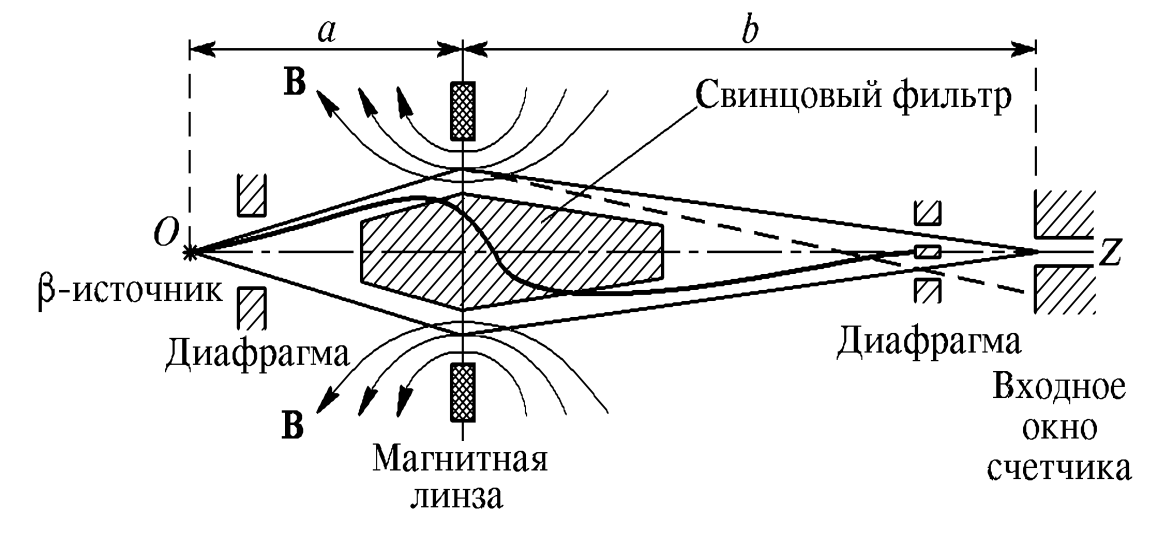
\includegraphics[width=0.7\linewidth]{Screenshot_2}
		\caption{Схема магнитной линзы}
		\label{fig:screenshot2}
	\end{figure}
	\begin{figure}
		\centering
		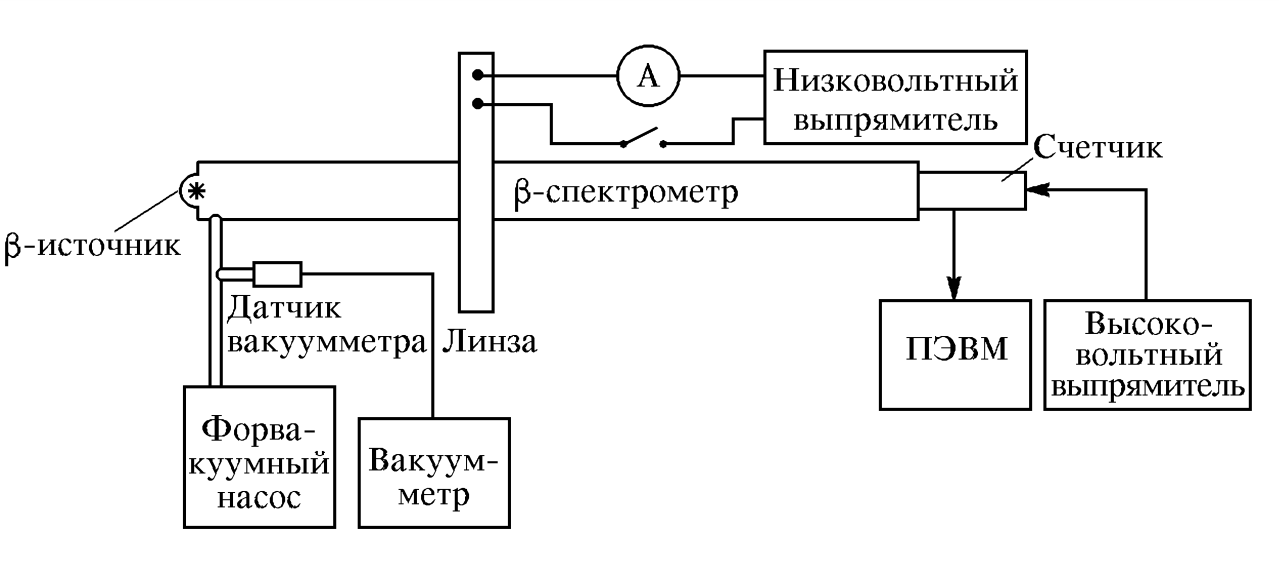
\includegraphics[width=0.7\linewidth]{Screenshot_3}
		\caption{Блок-схема экспериментальной установки}
		\label{fig:screenshot3}
	\end{figure}
	При заданной силе тока на входное окно счетчика фокусируются электроны с определенным импульсом. Электроны, обладающие другими значениями импульса, при этом не сфокусированы и в основном проходят мимо окна. При изменении тока в катушке на счетчик последовательно фокусируются электроны с разными	импульсами, то есть
	\begin{equation*}\label{eq:impulse}
		p_e = k I,
	\end{equation*}
	где $ I $ -- ток катушки.
	Для числа электронов, имеющих импульс $ p_e+\Delta p_e $, можно получить
	\begin{equation*}\label{eq:n_ot_Pe}
		N(p_e) = C W(p_e) p_e,
	\end{equation*}
	где $ C = \const $, $ W(p_e) = d w / d p_e $ находится из формулы \eqref{eq:simpleSpectre}.
	
	\newpage
	В работе используются:
	\begin{itemize}
		\equip{\btt-источник}
		\equip{Форвакуумный насос}
		\equip{Вакуумметр (фигура номинальная)}
		\equip{Магнитная линза со свинцовым фильтром и диафрагмой}
		\equip{Сцинтилляционный счётчик}
		\Equip{Источники питания}{0,02}{А}
		\equip{Компьютер}
	\end{itemize}
	
	\section{Результаты измерений и обработка данных}
	
	Проведём подробное измерение \btt-спектра, особенно в области конверсионного пика (энергия электронов внутренней конверсии	\isotope{Cs}{137} равна 634 кэВ).	Кроме того, измерим фон.
	
	На месте проведём предварительную обработку результатов эксперимента: учтём фон, прокалибруем спектрометр по конверсионному пику. Кроме того, построим график Ферми-Кюри.
	Полученные данные, с учётом погрешностей (об их оценке в \ref{sec:error}) находятся в табл. \ref{tab:raw}. 
	
	Построим два графика: $ N = F(J) $ на рис. \ref{fig:graph1} и $ \sqrt{N - N_ф}/p^{\frac{3}{2}}\left[мкФерми\right] = F(T) $	на рис.
	
	\begin{figure}[]
		\centering
		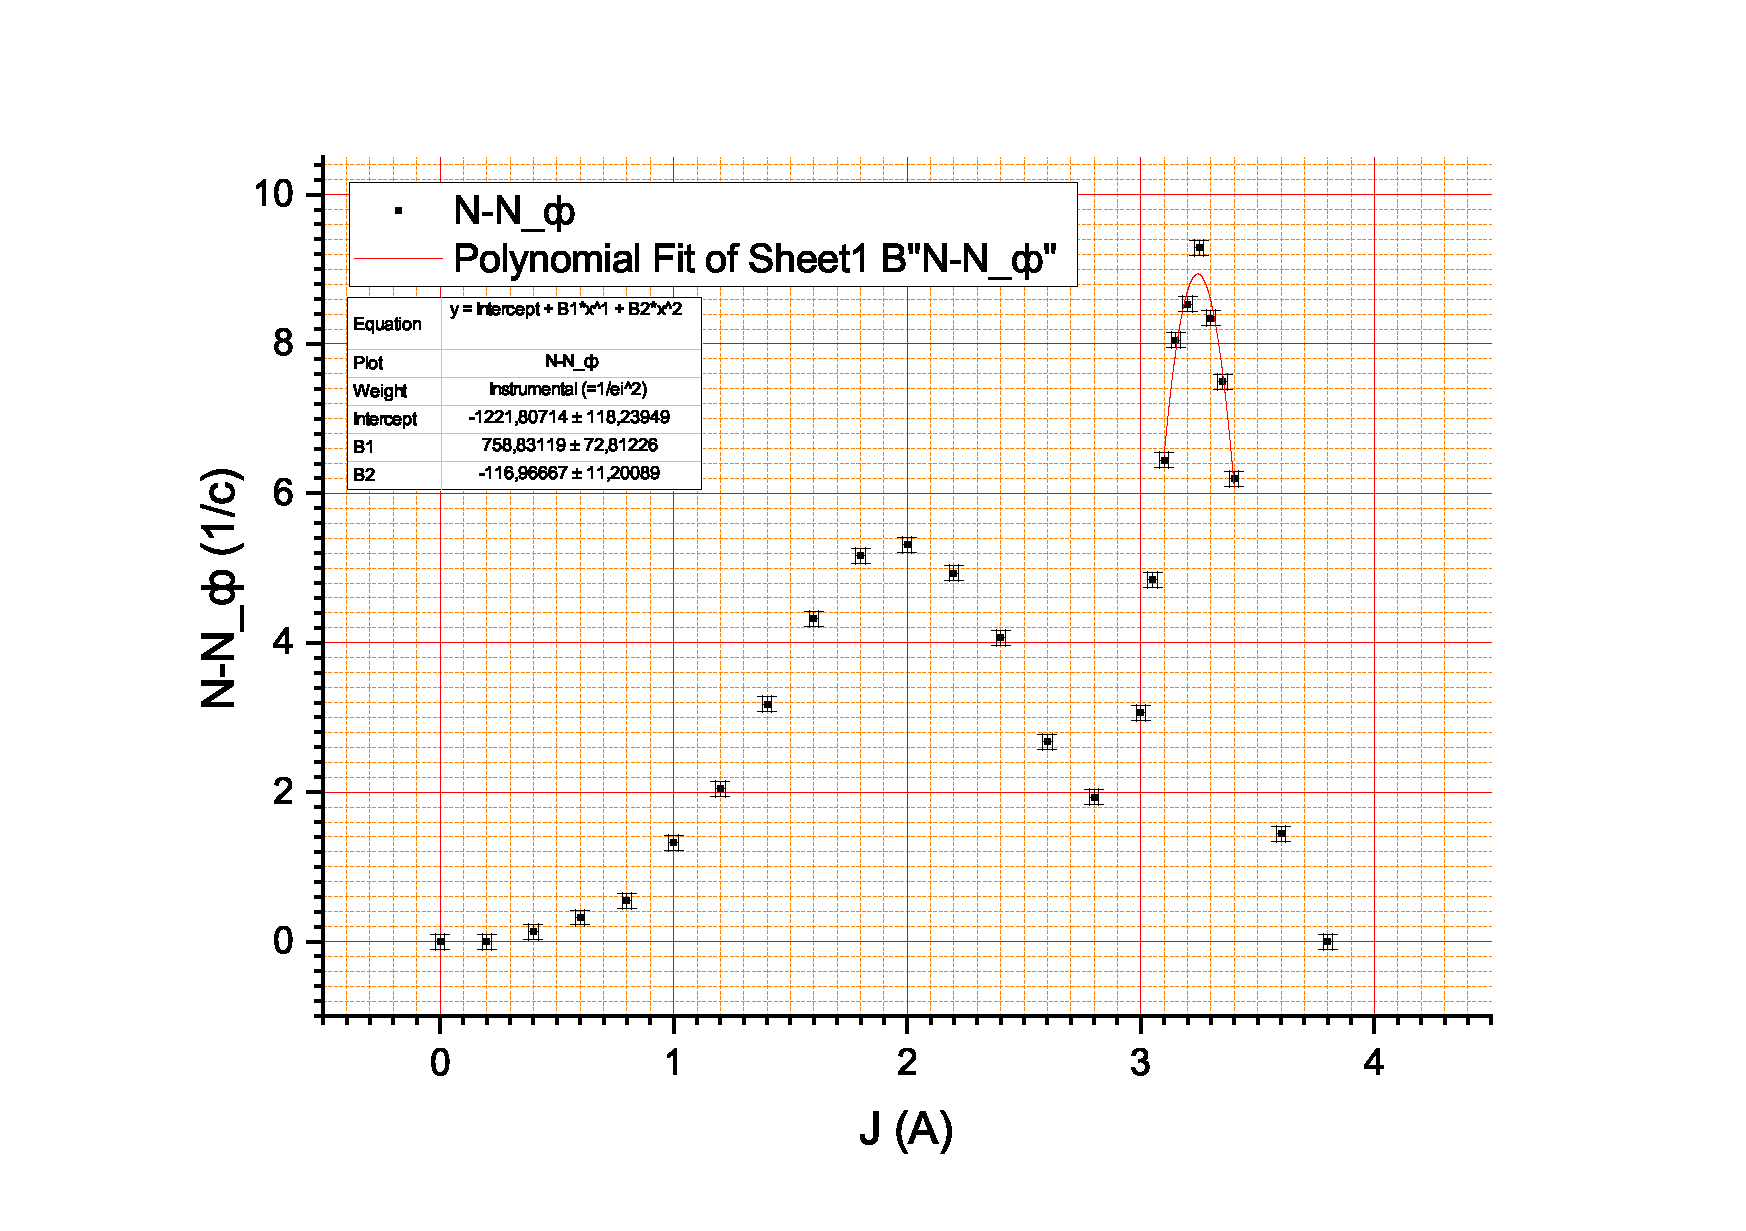
\includegraphics[width=0.9\linewidth]{Graph1}
		\caption{График зависимости числа частиц от тока $J$}
		\label{fig:graph1}
	\end{figure}
	
	\begin{figure}
		\centering
		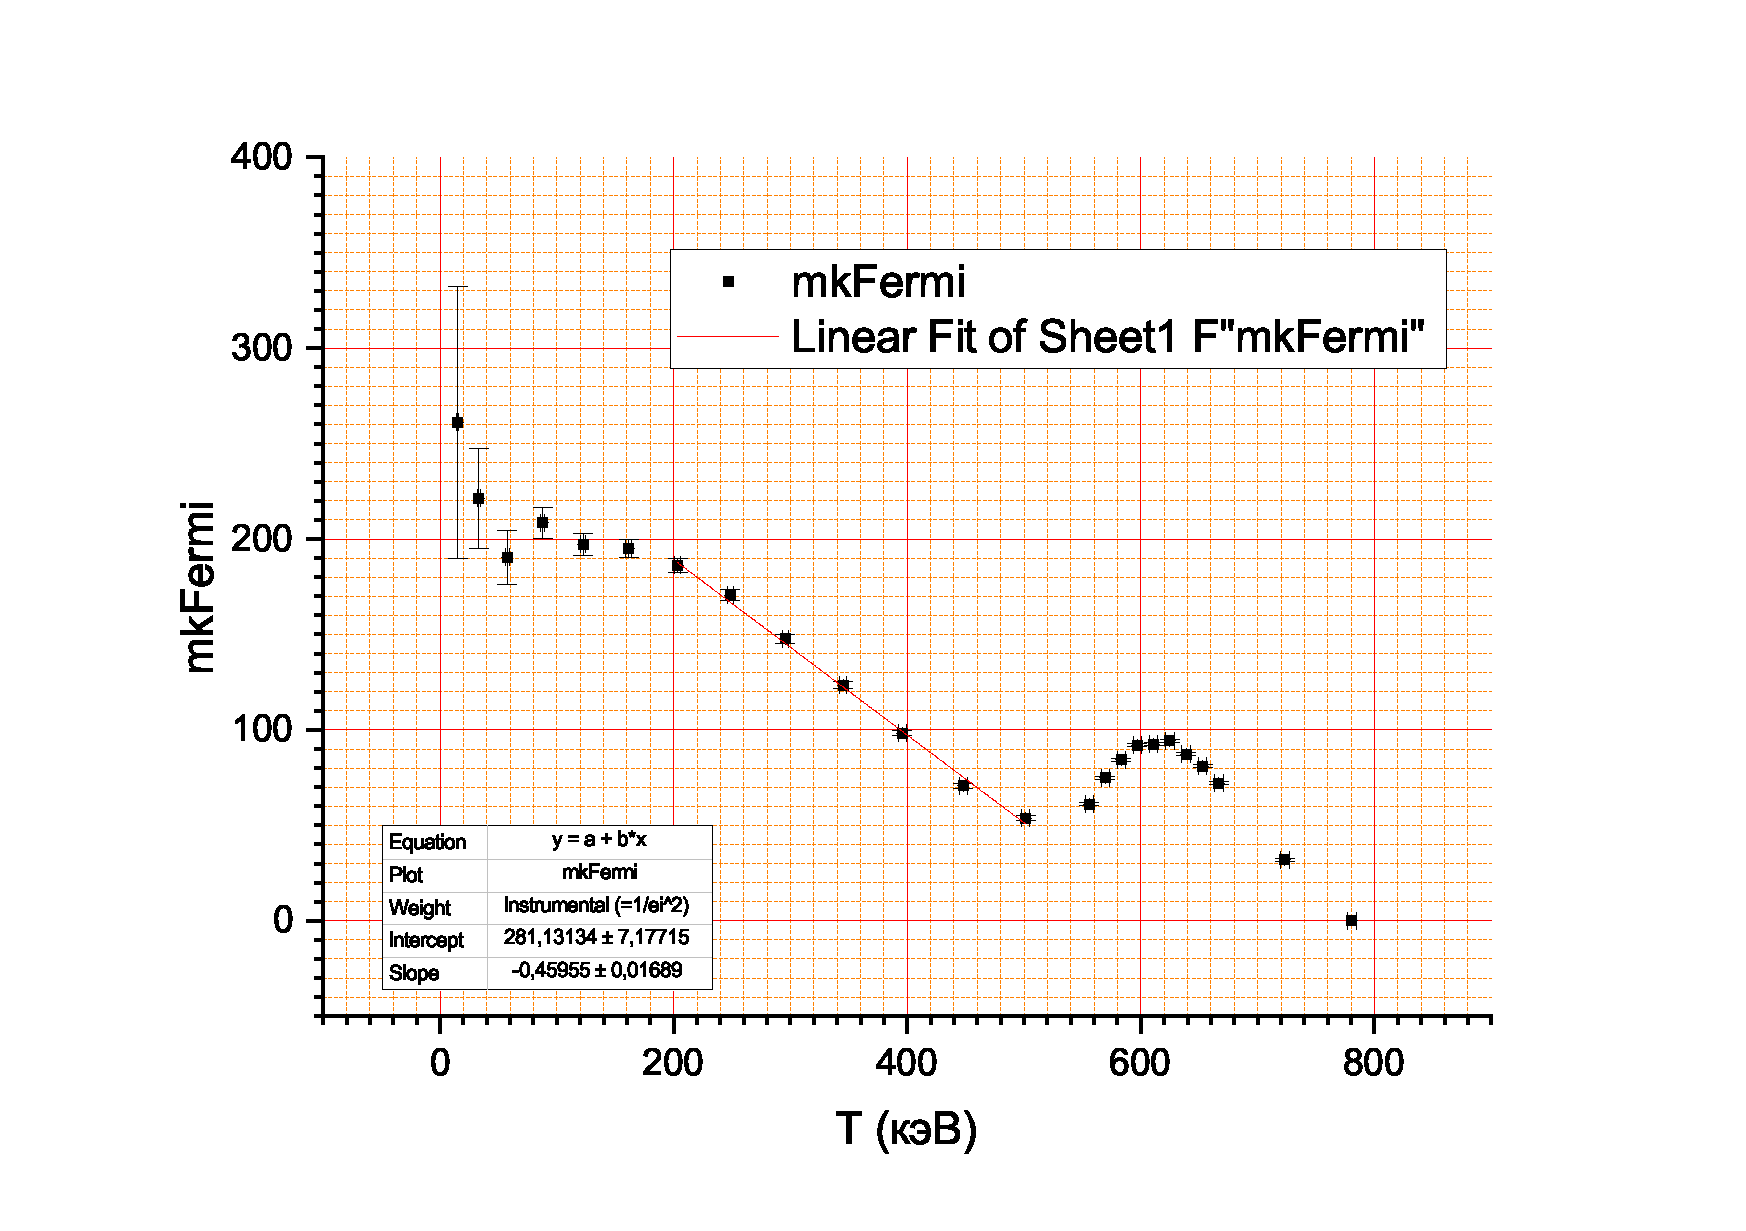
\includegraphics[width=0.9\linewidth]{Graph2}
		\caption{График Ферми-Кюри}
		\label{fig:graph2}
	\end{figure}
	
	Из первого графика видно, что пик имеет место практически точно при $ J = 3,25\; А $, значит, калибровка, проведённая на месте и данные таблицы \ref{tab:raw} заслуживают дальнейшего излучения.
	
	По второму графику, принимая во внимание только точки в средней части и экстраполируя полученную прямую до оси абсцисс, найдём граничную энергию \btt-спектра:
	\[E_\beta^\mathrm{max} = - \dfrac{a}{b} = 612\pm 4 \; кэВ.\]

	Стоит принять во внимание, что в экстраполяции принимала участие только центральная часть графика, так как данные начальной части имеют существенные погрешности и вообще не очень точны, так как малы энергии электронов, и начинает действовать сила Кулона. Конечная часть графика не выходит на прямую после конверсионного пика, так как блоки питания не могли дать достаточный ток, и крайние точки снять не удалось.
	
	\subsection{Оценка погрешностей}
		
		\label{sec:error}
		
	Точная оценка для величины $ N $, даже из статистических соображений, невозможна, так как во-первых, для каждого опыта сделано только одно измерение, а во-вторых, неизвестна инструментальная погрешность сцинтиллятора и установки в целом. Поэтому считаем погрешность величины $ N $ равной погрешности $ N_ф $, так как только её можно выяснить достаточно достоверно.
		
		\begin{equation*}\label{key}
			\sigma_{N_ф} = 0,04 \;c^{-1}.
		\end{equation*}
		
	Оценка косвенных погрешностей проводится при помощи пакета \emph{Wolfram Mathematica} по общей формуле:
	\begin{equation}\label{eq:погрешности}
		\Delta_{u(x, y, z, \ldots)}^2 = f'^2_{x} \Delta_x^2 + f'^2_y \Delta_y^2 + f'^2_z \Delta_z^2 + \ldots,
	\end{equation}
	
	Статистическая погрешность для среднего значения $ N_ф $ может быть вычислена по формуле стандартной ошибки среднего
	\begin{equation}\label{eq:stat}
		\sigma_{N_ф} = \sqrt{\dfrac{1}{n (n-1)} \sum_{i=1}^{n}\left( (N_ф)_i - N_ф \right)^2 }.
	\end{equation}
	
	\newpage
	\section{Вывод}
	
	По результатам работы изучили энергетический спектр \btt-частиц (см. рис. \ref{fig:graph3}); кроме того было получено значение максимальной энергии для электрона при \btt-распаде.
	\begin{figure}
		\centering
		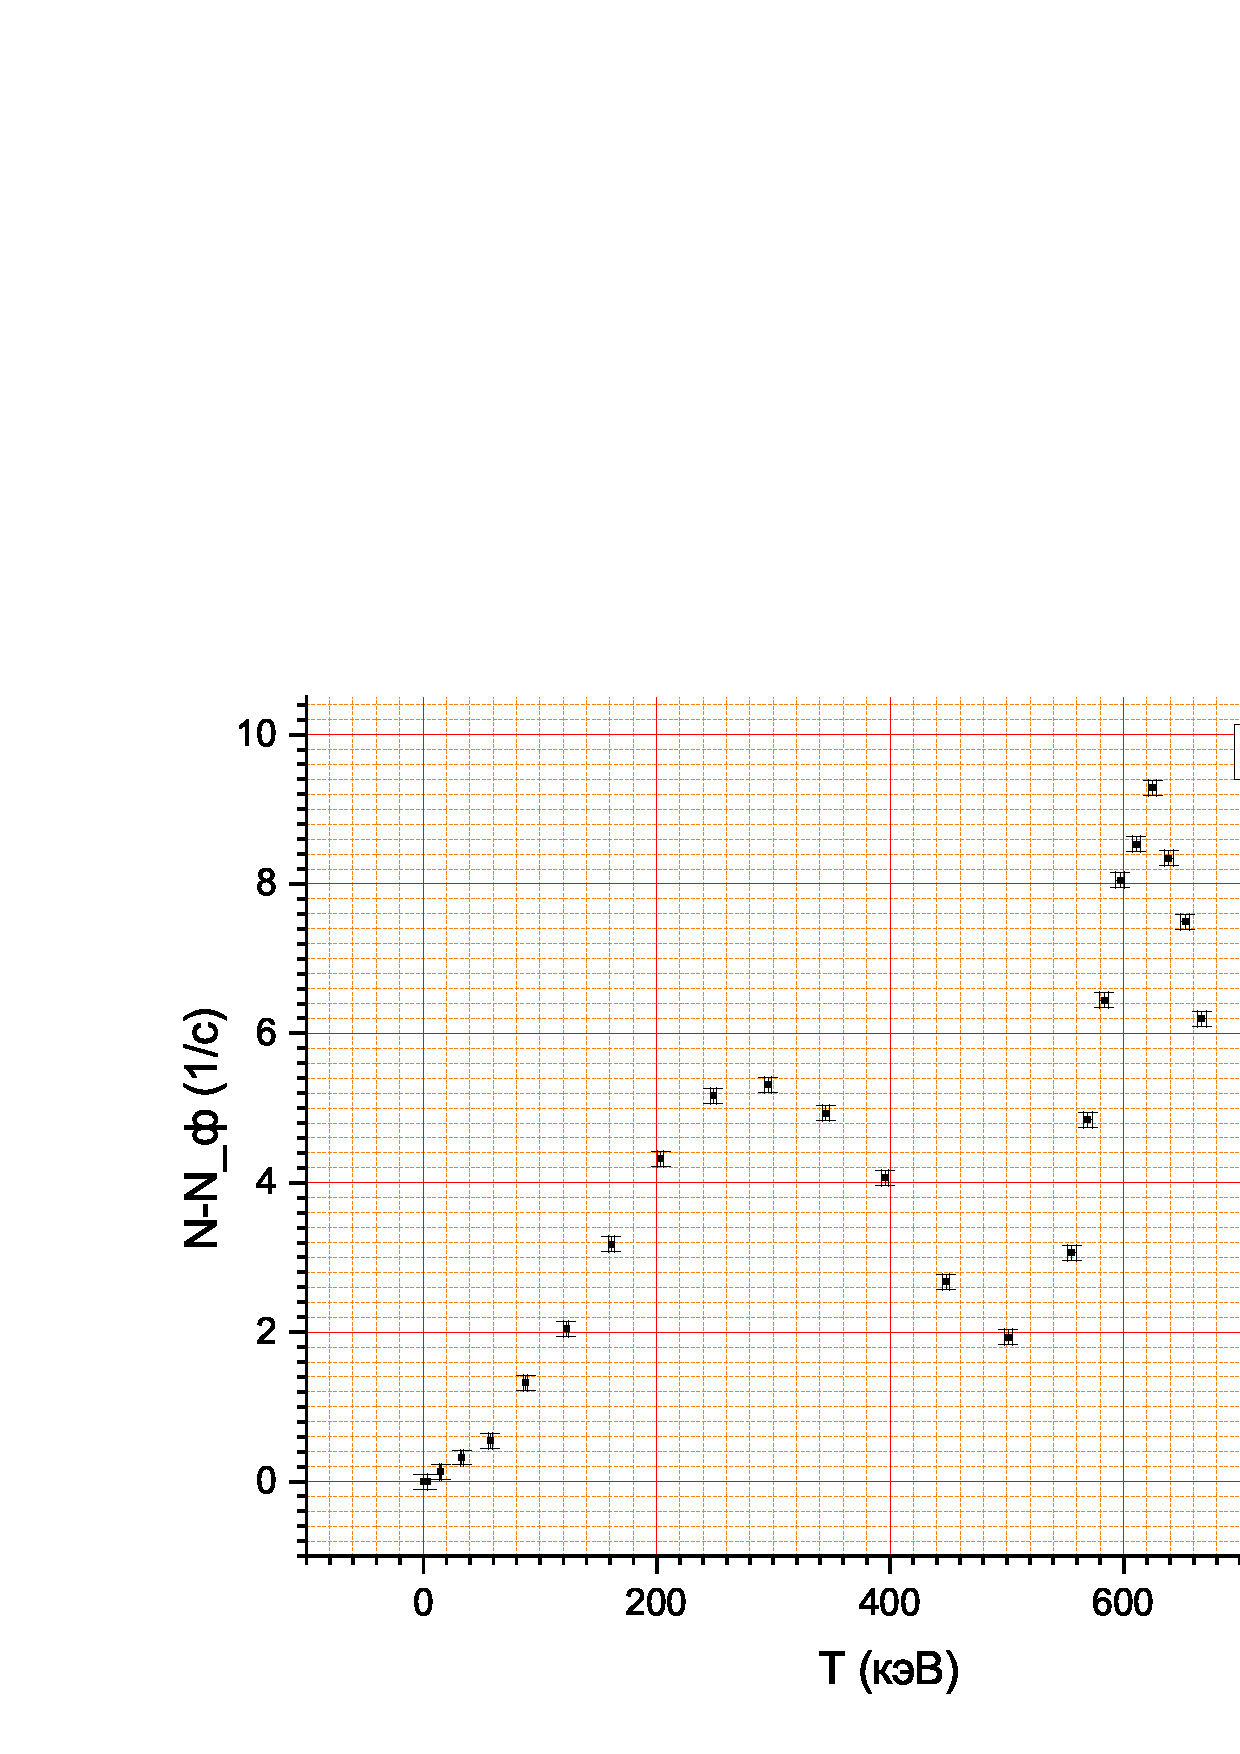
\includegraphics[width=0.9\linewidth]{Graph3}
		\caption{Спектр \btt-частиц (распределение по энергии)}
		\label{fig:graph3}
	\end{figure}
	
			\newpage
	\appendix
	\section{Необработанные результаты опытов}
	
	<<Сырые>> данные, полученные по результатам опытов, представлены в табл. \ref{tab:raw} и табл. \ref{tab:phone}.
	
% Please add the following required packages to your document preamble:
% \usepackage{multirow}
% Please add the following required packages to your document preamble:
% \usepackage{multirow}
\begin{table}[h]
	\centering
	\begin{tabular}{|l|l|l|l|l|l|l|l|l|l|}
		\hline
		$J, \;A$ &
		$\Delta J, \; A$ &
		$N$ &
		$\Delta_{N}$ &
		$p_e, \;кэВ / с$ &
		$\Delta p_e, \;кэВ/с$ &
		$T, \; кэВ$ &
		$\Delta T, \; кэВ$ &
		$mkFermi$ &
		$\Delta_{mkFermi}$ \\ \hline
		0,00 &
		\multirow{26}{*}{0,02} &
		0 &
		\multirow{26}{*}{0,07} &
		0 &
		\multirow{26}{*}{6} &
		0 &
		0 &
		0 &
		-- \\ \cline{1-1} \cline{3-3} \cline{5-5} \cline{7-10} 
		0,20 &  & 0    &  & 62   &  & 3,8   & 0,5 & 0      & --   \\ \cline{1-1} \cline{3-3} \cline{5-5} \cline{7-10} 
		0,40 &  & 0,13 &  & 124  &  & 15    & 1   & 261,27 & 71,3 \\ \cline{1-1} \cline{3-3} \cline{5-5} \cline{7-10} 
		0,60 &  &      &  & 187  &  & 33,2  & 1   & 221,37 & 26,3 \\ \cline{1-1} \cline{3-3} \cline{5-5} \cline{7-10} 
		0,80 &  & 0,54 &  & 246  &  & 57,7  & 1   & 190,35 & 14,1 \\ \cline{1-1} \cline{3-3} \cline{5-5} \cline{7-10} 
		1,00 &  & 1,32 &  & 312  &  & 87,8  & 2   & 208,53 & 8,2  \\ \cline{1-1} \cline{3-3} \cline{5-5} \cline{7-10} 
		1,20 &  & 2,04 &  & 374  &  & 122,6 & 2   & 197,19 & 5,8  \\ \cline{1-1} \cline{3-3} \cline{5-5} \cline{7-10} 
		1,40 &  & 3,17 &  & 437  &  & 161,4 & 2   & 195,11 & 4,6  \\ \cline{1-1} \cline{3-3} \cline{5-5} \cline{7-10} 
		1,60 &  & 4,32 &  & 499  &  & 203,5 & 2   & 186,26 & 3,7  \\ \cline{1-1} \cline{3-3} \cline{5-5} \cline{7-10} 
		1,80 &  & 5,16 &  & 561  &  & 248,5 & 3   & 170,67 & 3,0  \\ \cline{1-1} \cline{3-3} \cline{5-5} \cline{7-10} 
		2,00 &  & 5,30 &  & 624  &  & 295,7 & 3   & 147,71 & 2,3  \\ \cline{1-1} \cline{3-3} \cline{5-5} \cline{7-10} 
		2,20 &  & 4,93 &  & 686  &  & 345   & 3   & 123,41 & 1,8  \\ \cline{1-1} \cline{3-3} \cline{5-5} \cline{7-10} 
		2,40 &  & 4,06 &  & 749  &  & 395,8 & 3   & 98,34  & 1,5  \\ \cline{1-1} \cline{3-3} \cline{5-5} \cline{7-10} 
		2,60 &  & 2,67 &  & 811  &  & 448   & 3   & 70,76  & 1,2  \\ \cline{1-1} \cline{3-3} \cline{5-5} \cline{7-10} 
		2,80 &  & 1,93 &  & 874  &  & 501,4 & 3   & 53,81  & 1,1  \\ \cline{1-1} \cline{3-3} \cline{5-5} \cline{7-10} 
		3,00 &  & 3,06 &  & 936  &  & 555,8 & 3   & 61,11  & 0,9  \\ \cline{1-1} \cline{3-3} \cline{5-5} \cline{7-10} 
		3,05 &  & 4,84 &  & 952  &  & 569,5 & 4   & 74,92  & 0,9  \\ \cline{1-1} \cline{3-3} \cline{5-5} \cline{7-10} 
		3,10 &  & 6,44 &  & 967  &  & 583,3 & 4   & 84,33  & 0,9  \\ \cline{1-1} \cline{3-3} \cline{5-5} \cline{7-10} 
		3,15 &  & 8,05 &  & 983  &  & 597,1 & 4   & 92,05  & 0,9  \\ \cline{1-1} \cline{3-3} \cline{5-5} \cline{7-10} 
		3,20 &  & 8,13 &  & 998  &  & 611   & 4   & 90,33  & 0,9  \\ \cline{1-1} \cline{3-3} \cline{5-5} \cline{7-10} 
		3,25 &  & 9,28 &  & 1014 &  & 624,9 & 4   & 94,32  & 0,9  \\ \cline{1-1} \cline{3-3} \cline{5-5} \cline{7-10} 
		3,30 &  & 8,34 &  & 1030 &  & 638,8 & 4   & 87,36  & 0,8  \\ \cline{1-1} \cline{3-3} \cline{5-5} \cline{7-10} 
		3,35 &  & 7,49 &  & 1045 &  & 652,8 & 4   & 80,97  & 0,8  \\ \cline{1-1} \cline{3-3} \cline{5-5} \cline{7-10} 
		3,40 &  & 6,19 &  & 1061 &  & 666,9 & 4   & 72,01  & 0,7  \\ \cline{1-1} \cline{3-3} \cline{5-5} \cline{7-10} 
		3,60 &  & 1,44 &  & 1123 &  & 723,4 & 4   & 31,90  & 0,8  \\ \cline{1-1} \cline{3-3} \cline{5-5} \cline{7-10} 
		3,80 &  & 0    &  & 1186 &  & 780,5 & 4   & 0      & --   \\ \hline
	\end{tabular}
	\caption{Исходные данные (здесь $N = N - N_ф$)}
	\label{tab:raw}
\end{table}

	\begin{table}[h]
		\centering
		\begin{tabular}{|l|l|l|l|l|}
			\hline
			№             & 1     & 2     & 3     & 4     \\ \hline
			$N_ф, \; 1/c$ & 0,81 & 0,91 & 0,79 & 0,82 \\ \hline
		\end{tabular}
		\caption{Измерение фона}
		\label{tab:phone}
	\end{table}

	\begin{thebibliography}{3}
		\bibitem{Siv} Сивухин Д. В. \emph{Общий курс физики. Том 5}, 1989
		\bibitem{chp} Фаддеев М. А., Чупрунов Е. В. \emph{Лекции по атомной физике}, 2008
		\bibitem{tsip} Ципенюк Ю. М. \emph{Квантовая микро- и макрофизика}, 2006
		\bibitem{max} Игошин Ф. Ф., Самарский Ю. А., Ципенюк Ю. М. \emph{ЛАБОРАТОРНЫЙ ПРАКТИКУМ ПО ОБЩЕЙ ФИЗИКЕ. Квантовая физика: Учеб, пособие для вузов}; Под ред. Ципенюка Ю.М.
	\end{thebibliography}
\end{document}